\section{Introduction to Statistical Modelling}

Suppose we want to understand \textit{how much rainfall do we expect to get} on a particular day. We denote this \textbf{quantitative} variable as $Y$. Next, we make an assumption of what all parameters impact our variable $Y$. In this case, it could be \textit{temperature, humidity, wind speed, month of the year,} and so on. If our assumption is wrong, we will come to know about that during our analysis and modelling process. So, we can safely assume that there are $p$ measureable predictors that impact $Y$ and could be denoted by $X_1$, $X_2$, $X_3$,...,$X_p$.  Let $X$ be the set of all these predictors: $X = (X_1, X_2, X_3, ..., X_p)$. We want to find the \textbf{unknown} function $f$ such that

\[
Y = f(X) + \epsilon
\]

where $\epsilon$ is the error term. \textit{Why do we have an error term?} Because even the best models can’t capture every tiny detail of reality. There’s always some randomness, some noise, or some missing information. Epsilon accounts for all the stuff we don't know, couldn’t measure or predict.\\

Usually, we have some historic measurements of $Y$ and the corresponding values of $X$. By looking at these measurements, we try to come up with a function $\hat{f}$ which is an estimate of the original unknown function $f$. This will give us $\hat{Y}$, our prediction/estimate of the $Y$. 

\[
\hat{Y} = \hat{f}(X)
\]

We still don't know how we will come up with this $\hat{f}$ function. For us, it is a \textit{black box}, in the sense that one is not typically concerned with the exact form of $\hat{f}$, provided that it yields accurate predictions for $Y$.\cite{islr}\\

The accuracy of $\hat{Y}$ as an estimate for $Y$ relies on two main sources of error: the \textit{reducible error} and the \textit{irreducible error}. Generally, $\hat{f}$, which is our estimate of $f$, is not perfect, leading to some inaccuracies. This discrepancy contributes to the \textit{reducible error} because it can potentially be minimized by selecting a more suitable statistical learning method to estimate $f$. \\

However, even if we could perfectly estimate $f$ so that our prediction is $\hat{Y} = f(X)$, there would still be some inherent error present. This is because $Y$ depends not only on $f(X)$ but also on a random error term, $\epsilon$, which by its nature cannot be predicted using $X$. The uncertainty introduced by $\epsilon$ affects the accuracy of our predictions, and this is referred to as the \textit{irreducible error}, as it cannot be reduced, regardless of how accurately we estimate $f$.\\

Why is the irreducible error greater than zero? The term $\epsilon$ may contain unobserved variables that could help in predicting $Y$; since these variables are not measured, $f$ cannot utilize them for prediction. Additionally, $\epsilon$ may also account for random variation that cannot be measured. For instance, a patient’s risk of an adverse reaction could vary from day to day based on variations in the drug’s manufacturing process or the patient’s overall health status.\\

Now, consider an estimate $\hat{f}$ and a set of predictors $X$ which yield the prediction $\hat{Y} = \hat{f}(X)$. Assume that $\hat{f}$ and $X$ are fixed for a moment. Then, we can express the expected squared error as follows:

\begin{equation}
    E[(Y - \hat{Y})^2] = E[(f(X) + \epsilon - \hat{f}(X))^2] = [f(X) - \hat{f}(X)]^2 + \text{Var}(\epsilon)
\end{equation}
\vspace{3pt}

Here, $E[(Y - \hat{Y})^2]$ denotes the expected value of the squared difference between the predicted and actual values of $Y$, which is also called the mean squared error (MSE). The term $\text{Var}(\epsilon)$ represents the variance of the error term $\epsilon$. \\

The focus of this discussion is on methods to estimate $f$ with the goal of minimizing the reducible error. However, it is crucial to remember that the irreducible error sets an upper limit on the accuracy of our predictions for $Y$. This upper bound is often unknown in practice.\\

\subsection{How to estimate $\hat{f}$}\cite{islr}

Throughout this book, we discuss various linear and non-linear techniques for estimating the function $f$. Although these methods differ, they tend to share some common features, which we will outline in this section. We assume that we have observed a collection of $n$ data points. These observations are known as the \textit{training data} because they are used to train or teach our method to estimate the function $f$. Let $x_{ij}$ denote the value of the $j$th predictor (or input) for the $i$th observation, where $i = 1, 2, \ldots, n$ and $j = 1, 2, \ldots, p$. Let $y_i$ represent the response variable for the $i$th observation. Thus, our training data can be expressed as:

\[
\{(x_1, y_1), (x_2, y_2), \ldots, (x_n, y_n)\}
\]

where $x_i = (x_{i1}, x_{i2}, \ldots, x_{ip})^T$. Our objective is to apply a statistical learning method to this training data to estimate the unknown function $f$. In essence, we aim to find a function $\hat{f}$ such that $Y \approx \hat{f}(X)$ for any new observation $(X, Y)$. Generally, most statistical learning approaches for this task fall into one of two categories: \textit{parametric} or \textit{non-parametric}.

\subsubsection{Parametric Methods}

Parametric methods rely on a two-step model-based process:

\begin{enumerate}
    \item \textbf{Assume a Functional Form}: We start by making an assumption about the form or structure of $f$. For instance, a straightforward assumption is that $f$ is linear in $X$, leading to a model of the form:

    \[
    f(X) = \beta_0 + \beta_1 X_1 + \beta_2 X_2 + \ldots + \beta_p X_p
    \]

    This is known as a linear model, which we will explore in detail throughout this book. By assuming $f$ is linear, the task of estimating $f$ becomes much simpler. Instead of estimating an entirely arbitrary function in a $p$-dimensional space, we now only need to estimate $p + 1$ coefficients: $\beta_0, \beta_1, \ldots, \beta_p$.

    \item \textbf{Fitting the Model}: Once the model form is selected, the next step involves fitting or training the model using the training data. In the case of the linear model mentioned above, we need to estimate the parameters $\beta_0, \beta_1, \ldots, \beta_p$ in such a way that:

    \[
    Y \approx \beta_0 + \beta_1 X_1 + \beta_2 X_2 + \ldots + \beta_p X_p
    \]

    The most common method for fitting such a model is \textit{ordinary least squares}. This approach minimizes the squared differences between the observed values and the values predicted by the model. However, ordinary least squares is just one way to fit a linear model; there are several alternative methods depending on the problem.
\end{enumerate}

The parametric approach described reduces the problem of estimating $f$ to estimating a finite set of parameters. By assuming a specific form for $f$, the estimation process becomes more manageable, as it typically involves fewer variables. However, a significant drawback of this approach is that the model chosen might not align closely with the true underlying function $f$. If the assumed model is too restrictive or too far from reality, our estimate will not be accurate. To mitigate this, we can opt for more flexible parametric models that capture a wider range of possible functional forms for $f$. Nevertheless, increasing the flexibility of a model generally requires estimating more parameters, which can lead to \textit{overfitting}. Overfitting occurs when the model captures the noise in the training data rather than the actual underlying pattern, leading to poor performance on new, unseen data.

\subsubsection{Non-parametric Methods}

Non-parametric methods take a different approach by avoiding explicit assumptions about the functional form of $f$. Instead, these methods aim to estimate $f$ directly from the data, adjusting to fit the data points as closely as possible without becoming overly complex or erratic. One of the major advantages of non-parametric methods is that they offer the flexibility to fit a broad range of shapes for $f$. By not imposing a specific form, these methods can potentially provide a more accurate estimate, particularly when the true function $f$ is complex or unknown.\\

However, this flexibility comes at a cost. Because non-parametric methods do not simplify the problem to a set of parameters, they typically require a much larger number of observations compared to parametric methods in order to produce a reliable estimate. Essentially, they need a rich dataset to accurately capture the patterns in the data without resorting to assumptions about the functional form of $f$.

\subsection{Measuring the Quality of the Model}

In modelling, the Mean Squared Error (MSE) is a fundamental measure used to assess the performance of models. It quantifies the average squared difference between the actual values and the predicted values. Specifically, the MSE is defined as:

\[
\text{MSE} = \frac{1}{n} \sum_{i=1}^{n} (y_i - \hat{y}_i)^2
\]

where \( y_i \) are the observed values, \( \hat{y}_i \) are the predicted values, and \( n \) is the number of observations. To evaluate the effectiveness of a model, it is common practice to split the data into two parts: the training set and the test set. The MSE calculated using these two subsets is referred to as the \textit{Training MSE} and \textit{Test MSE}, respectively.\\

\textbf{Training MSE} measures how well a model fits the data it was trained on. It is the average squared error computed using the training dataset. On the other hand, \textbf{Test MSE} evaluates the model's performance on unseen data, providing insight into how the model is expected to perform in practice.\\

As a general rule, \textit{the training MSE will decrease as the complexity (or flexibility) of the model increases}. When the model becomes more flexible, it can fit the training data more closely. In other words, a highly flexible model is capable of capturing the intricate details and patterns of the training dataset, resulting in a lower training MSE.\\

However, the test MSE may not necessarily decrease as model flexibility increases. In fact, it might initially decrease but will eventually increase, forming what is known as a \textbf{U-shape} curve. This phenomenon occurs due to the concept of \textbf{overfitting}.

\subsubsection{The U-Shape Curve of Test MSE}

When a model is overly complex, it can fit the noise and peculiarities in the training data rather than the true underlying patterns. This situation leads to a scenario where the \textit{Training MSE} is very low, but the \textit{Test MSE} is high. This discrepancy indicates that the model has memorized the training data rather than learning a generalizable pattern. We say the model is \textbf{overfit}.\\

The U-shape of the test MSE can be explained as follows: 

\begin{itemize}
    \item When the model is \textit{underfitting} (i.e., it is too simple to capture the relationship between the predictors and the response), both the training and test MSEs are high.
    \item As we increase the flexibility of the model, it starts capturing more of the pattern, causing the training MSE and test MSE to drop.
    \item However, if we continue to increase the flexibility, the model becomes so attuned to the training data that it loses its ability to generalize. Consequently, the \textit{test MSE} rises, while the \textit{training MSE} continues to fall.
\end{itemize}

The following plot shows the relationship between the training and test MSE as model flexibility increases. The training MSE steadily decreases as the model becomes more flexible, while the test MSE initially decreases but eventually rises, forming a U-shape.

\begin{center}
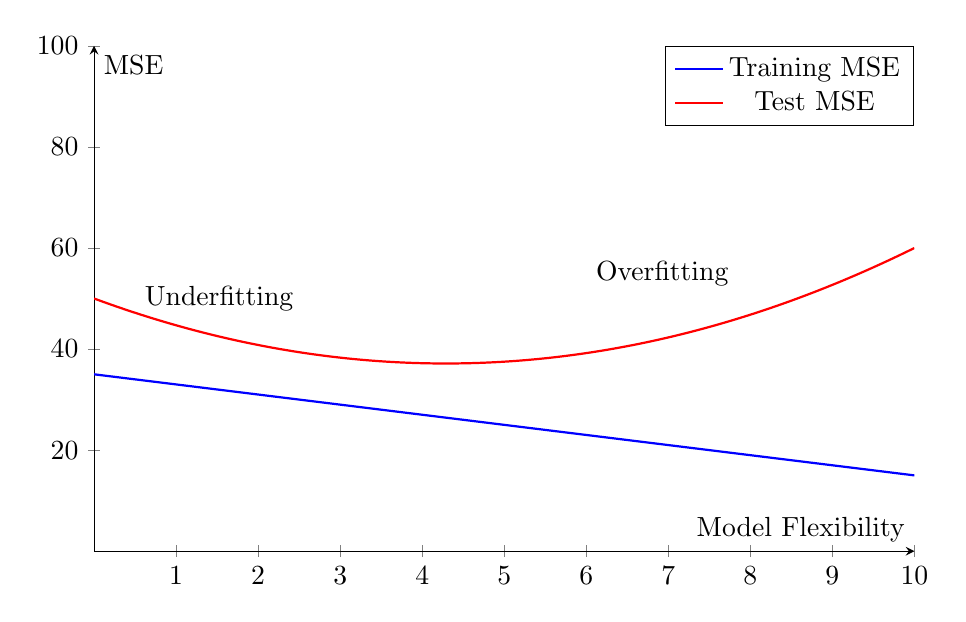
\begin{tikzpicture}
    \begin{axis}[
        xlabel={Model Flexibility},
        ylabel={MSE},
        ymin=0,
        xmin=0,
        xmax=10,
        ymax=100,
        legend style={at={(1,1)}, anchor=north east},
        domain=0:10,
        samples=100,
        axis x line=middle,
        axis y line=middle,
        width=12cm,
        height=8cm,
    ]
    % Training MSE curve
    \addplot [
        domain=0:10,
        smooth,
        thick,
        blue
    ] {35 - 2*x};
    \addlegendentry{Training MSE}

    % Test MSE curve
    \addplot [
        domain=0:10,
        smooth,
        thick,
        red
    ] {50 - 6*x + 0.7*x^2};
    \addlegendentry{Test MSE}

    % Annotations
    \node at (axis cs: 0.5,50) [anchor=west] {Underfitting};
    \node at (axis cs: 6,55) [anchor=west] {Overfitting};

    \end{axis}
\end{tikzpicture}
\end{center}

An important concept related to the train and test MSE is \textbf{variability}, or the sensitivity of a model to changes in the training data. A flexible model has higher variability, meaning it can change drastically with slight variations in the dataset. This makes it more likely to fit the noise in the data rather than the underlying pattern.\\

For example, if you were trying to predict house prices based on features like the number of bedrooms, location, and age of the house, a simple model might just give you a rough average price based on the number of bedrooms. While it may not be perfect, it would be relatively stable. In contrast, a very flexible model might try to fit every single fluctuation in price, even if those fluctuations are random or due to factors you haven’t measured. This model would perform extremely well on the training data but poorly on the test data because it would struggle with new, unseen examples that don't fit the training patterns precisely.

\section{Bias-Variance Trade Off}

Understanding the sources of error is critical for building models that generalize well to new data. One of the key concepts in this regard is the \textbf{bias-variance tradeoff}. It explains the balance between two sources of error that affect the performance of a model: \textbf{bias} and \textbf{variance}. These components together, along with irreducible error, make up the total prediction error. We express this relationship with the following equation:

\[
\mathbb{E} \left[ (y_0 - \hat{f}(x_0))^2 \right] = \text{Var}(\hat{f}(x_0)) + [\text{Bias}(\hat{f}(x_0))]^2 + \text{Var}(\epsilon)
\]

where:\\
 \( y_0 \) is the true output value at a new point \( x_0 \),\\
 \( \hat{f}(x_0) \) is the predicted value from the model at \( x_0 \),\\
 \( \text{Var}(\hat{f}(x_0)) \) is the variance of the model predictions at \( x_0 \),\\
 \( \text{Bias}(\hat{f}(x_0)) \) represents the bias of the model at \( x_0 \),\\
 \( \text{Var}(\epsilon) \) is the irreducible error, representing noise in the system that cannot be eliminated.

\subsubsection{Bias}

\textit{Bias} refers to the error introduced when the model oversimplifies the relationship between the predictors \( X \) and the response \( Y \). A model with high bias pays little attention to the details and patterns in the data, leading to inaccurate predictions. This typically happens when the model is too rigid or has low flexibility. In other words, it makes strong assumptions about the form of the relationship, like assuming a linear pattern when the actual relationship might be more complex.\\

An example of high bias is using a linear model to predict a highly non-linear relationship, such as trying to fit a straight line through data that clearly forms a parabolic pattern. Such a model will consistently miss the target values, resulting in a systematic error.\\

The squared bias term in the equation, \( [\text{Bias}(\hat{f}(x_0))]^2 \), measures the extent to which the average prediction of the model differs from the true value. High bias means the model is \textit{underfitting} the data.

\subsubsection{Variance}

\textit{Variance} refers to the model's sensitivity to small fluctuations in the training data. A model with high variance is overly complex and captures not just the underlying pattern but also the random noise in the training set. This leads to inconsistency when the model is applied to new, unseen data, as it produces vastly different outputs depending on the training data used.\\

Imagine a situation where you use a very flexible model, like a polynomial of high degree, to fit a dataset. The model will fit the training data almost perfectly, but if you change the training data slightly, the model's predictions could change drastically. This high sensitivity indicates that the model is not learning the general pattern but is instead learning the noise specific to the training data.\\

The term \( \text{Var}(\hat{f}(x_0)) \) in the equation represents this variability in the model's prediction at \( x_0 \). High variance means the model is \textit{overfitting} the data.

\subsubsection{The Bias-Variance Trade Off}

As we increase model flexibility, bias typically decreases because the model becomes capable of fitting more complex patterns. However, variance increases as the model starts capturing more noise from the training data. The goal is to find the \textbf{sweet spot} where the model is sufficiently complex to capture the underlying structure but not so flexible that it fits the noise. This is the point where the sum of bias and variance is minimized.\\

The term \( \text{Var}(\epsilon) \) in the equation represents the irreducible error or noise inherent in the system. No matter how well a model is designed, this error cannot be eliminated because it arises from factors beyond our control or measurement error in the observations.

\begin{figure}[h!]
    \centering
    \includegraphics[width=0.9\textwidth]{chapters/chapter1/plots/scatter_plot.png}
    \caption{Scatter Plot of CGPA vs Salary Package}
    \label{fig:scatter_plot}
\end{figure}